\chapter*{Prefacio}
Este documento es un trabajo de investigación para la asignatura ``\textit{Métodos algorítmicos en resolución de problemas}'', impartida por Narciso Martí Oliet y Clara María Segura Díaz en el curso $2018$--$2019$ al curso de tercero del doble grado de Ingeniería Informática -- Matemáticas en la Facultad de Informática de la Universidad Complutense de Madrid (UCM).

\subsection*{Contenido}
Este texto contiene una implementación detallada de los montículos $n$--arios y establece un estudio comparativo entre los diferentes costes de dichas estructuras.
\newline

Las palabras resaltadas con \textcolor{hyperlinkColour}{este color} contienen hipervínculos.

\subsection*{Licencia}
Esta obra está sujeta a la licencia Reconocimiento-NoComercial-CompartirIgual 4.0 Internacional de Creative Commons. Para ver una copia de esta licencia, visite \url{http://creativecommons.org/licenses/by-nc-sa/4.0/}.
\begin{figure}[h]
	\centering
	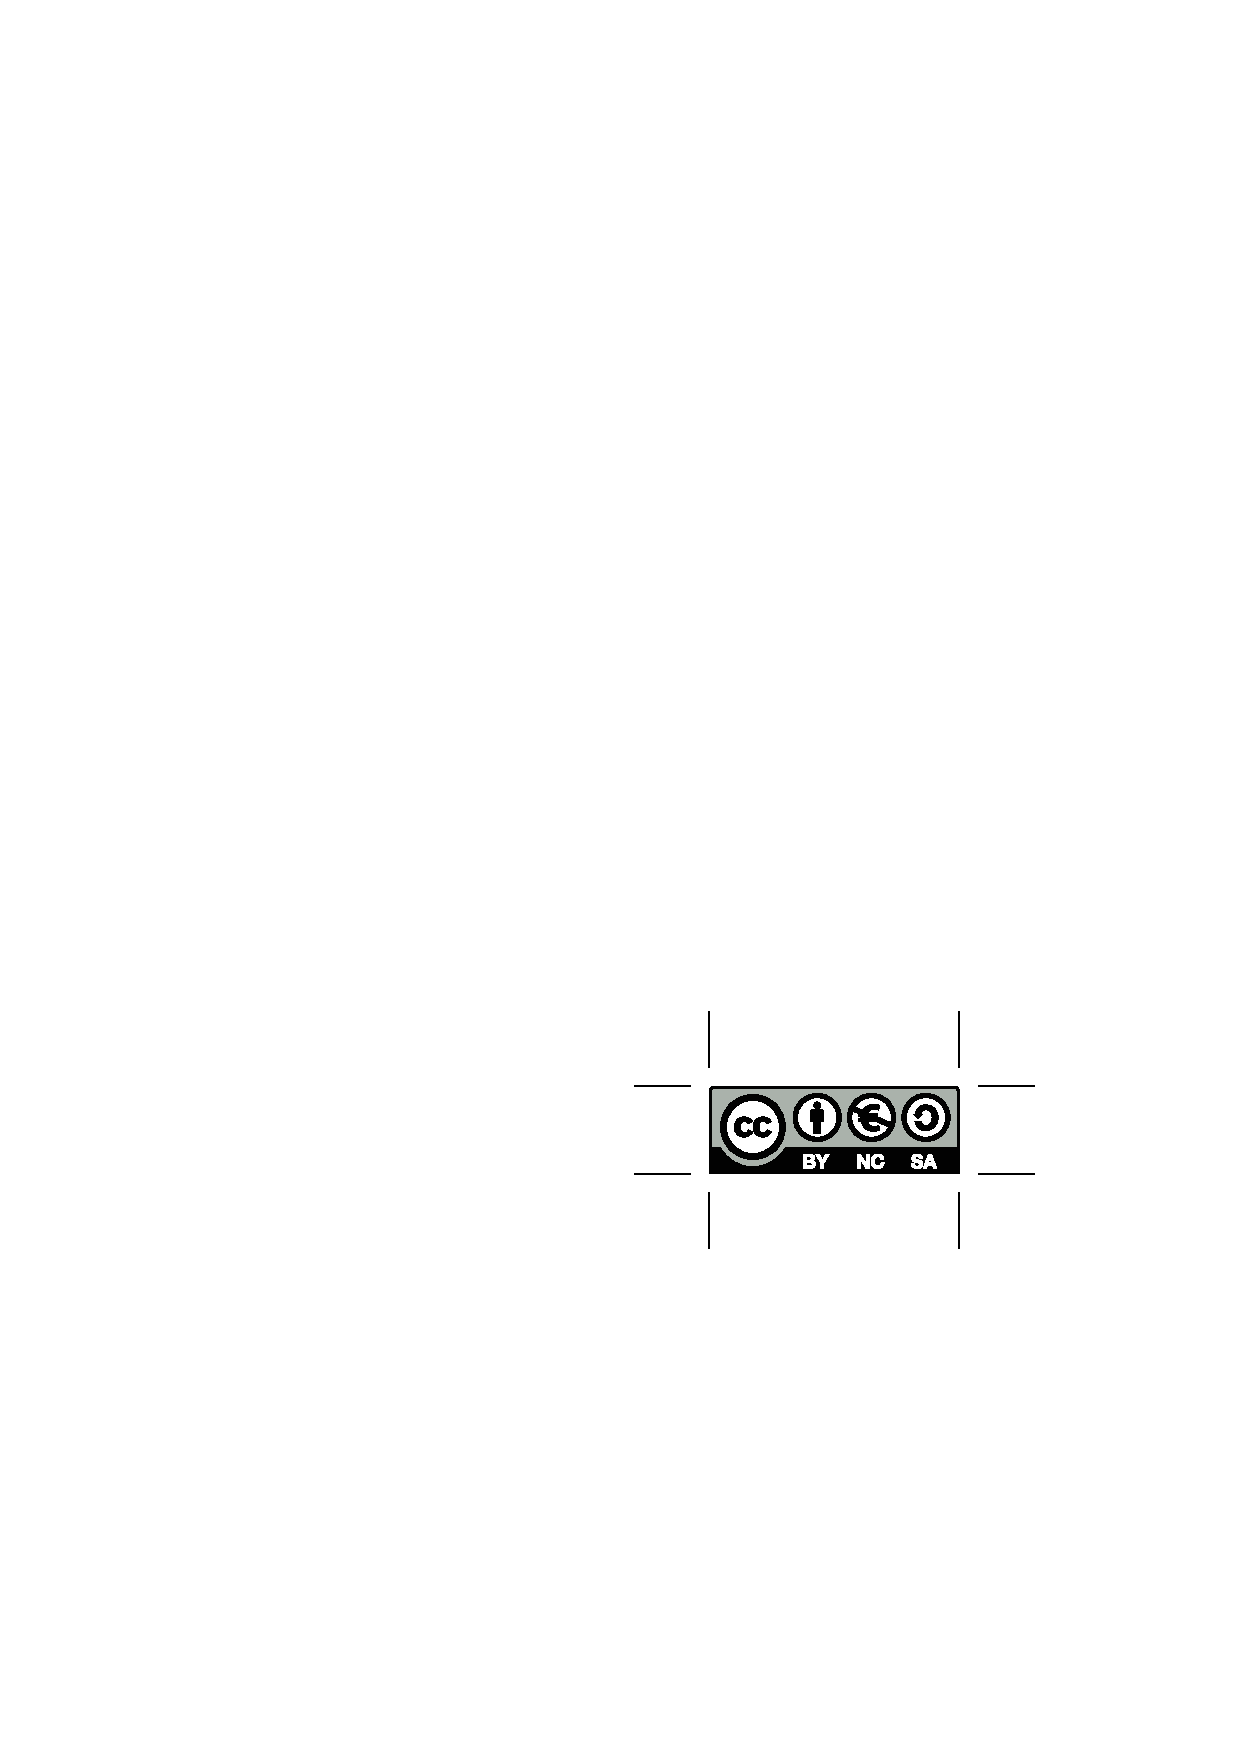
\includegraphics[scale=1]{img/licencia}
\end{figure}

El código fuente de este documento, así como el código de la implementación de los montículos $n$--arios, es de libre acceso y se encuentra alojado en \url{https://github.com/Inmapg/d-ary-heaps} paro uso y disfrute de todo el que quiera, siempre que se respeten los términos de la licencia.